\documentclass[a4paper]{article}
\usepackage[a4paper, margin=1in]{geometry}
% Some basic packages
\usepackage[utf8]{inputenc}
\usepackage[T1]{fontenc}
\usepackage{textcomp}
\usepackage[dutch]{babel}
\usepackage{url}
\usepackage{graphicx}
\usepackage{float}
\usepackage{booktabs}
\usepackage{enumitem}

\pdfminorversion=7

% Don't indent paragraphs, leave some space between them
\usepackage{parskip}

% Hide page number when page is empty
\usepackage{emptypage}
\usepackage{subcaption}
\usepackage{multicol}
\usepackage{xcolor}

% Other font I sometimes use.
% \usepackage{cmbright}

% Math stuff
\usepackage{amsmath, amsfonts, mathtools, amsthm, amssymb}
% Fancy script capitals
\usepackage{mathrsfs}
\usepackage{cancel}
% Bold math
\usepackage{bm}
% Some shortcuts
\newcommand\N{\ensuremath{\mathbb{N}}}
\newcommand\R{\ensuremath{\mathbb{R}}}
\newcommand\Z{\ensuremath{\mathbb{Z}}}
\renewcommand\O{\ensuremath{\emptyset}}
\newcommand\Q{\ensuremath{\mathbb{Q}}}
\newcommand\C{\ensuremath{\mathbb{C}}}

% Easily typeset systems of equations (French package)
\usepackage{systeme}

% Put x \to \infty below \lim
\let\svlim\lim\def\lim{\svlim\limits}

%Make implies and impliedby shorter
\let\implies\Rightarrow
\let\impliedby\Leftarrow
\let\iff\Leftrightarrow
\let\epsilon\varepsilon

% Add \contra symbol to denote contradiction
\usepackage{stmaryrd} % for \lightning
\newcommand\contra{\scalebox{1.5}{$\lightning$}}

% \let\phi\varphi

% Command for short corrections
% Usage: 1+1=\correct{3}{2}

\definecolor{correct}{HTML}{009900}
\newcommand\correct[2]{\ensuremath{\:}{\color{red}{#1}}\ensuremath{\to }{\color{correct}{#2}}\ensuremath{\:}}
\newcommand\green[1]{{\color{correct}{#1}}}

% horizontal rule
\newcommand\hr{
    \noindent\rule[0.5ex]{\linewidth}{0.5pt}
}

% hide parts
\newcommand\hide[1]{}

% si unitx
\usepackage{siunitx}
\sisetup{locale = FR}

% Environments
\makeatother
% For box around Definition, Theorem, \ldots
\usepackage{mdframed}
\mdfsetup{skipabove=1em,skipbelow=0em}
\theoremstyle{definition}
\newmdtheoremenv[nobreak=true]{definitie}{Definitie}
\newmdtheoremenv[nobreak=true]{eigenschap}{Eigenschap}
\newmdtheoremenv[nobreak=true]{gevolg}{Gevolg}
\newmdtheoremenv[nobreak=true]{lemma}{Lemma}
\newmdtheoremenv[nobreak=true]{propositie}{Propositie}
\newmdtheoremenv[nobreak=true]{stelling}{Stelling}
\newmdtheoremenv[nobreak=true]{wet}{Wet}
\newmdtheoremenv[nobreak=true]{postulaat}{Postulaat}
\newmdtheoremenv{conclusie}{Conclusie}
\newmdtheoremenv{toemaatje}{Toemaatje}
\newmdtheoremenv{vermoeden}{Vermoeden}
\newtheorem*{herhaling}{Herhaling}
\newtheorem*{intermezzo}{Intermezzo}
\newtheorem*{notatie}{Notatie}
\newtheorem*{observatie}{Observatie}
\newtheorem*{oef}{Oefening}
\newtheorem*{opmerking}{Opmerking}
\newtheorem*{praktisch}{Praktisch}
\newtheorem*{probleem}{Probleem}
\newtheorem*{terminologie}{Terminologie}
\newtheorem*{toepassing}{Toepassing}
\newtheorem*{uovt}{UOVT}
\newtheorem*{vb}{Voorbeeld}
\newtheorem*{vraag}{Vraag}

\newmdtheoremenv[nobreak=true]{definition}{Definition}
\newtheorem*{eg}{Example}
\newtheorem*{notation}{Notation}
\newtheorem*{previouslyseen}{As previously seen}
\newtheorem*{remark}{Remark}
\newtheorem*{note}{Note}
\newtheorem*{problem}{Problem}
\newtheorem*{observe}{Observe}
\newtheorem*{property}{Property}
\newtheorem*{intuition}{Intuition}
\newmdtheoremenv[nobreak=true]{prop}{Proposition}
\newmdtheoremenv[nobreak=true]{theorem}{Theorem}
\newmdtheoremenv[nobreak=true]{corollary}{Corollary}

% End example and intermezzo environments with a small diamond (just like proof
% environments end with a small square)
\usepackage{etoolbox}
\AtEndEnvironment{vb}{\null\hfill$\diamond$}%
\AtEndEnvironment{intermezzo}{\null\hfill$\diamond$}%
% \AtEndEnvironment{opmerking}{\null\hfill$\diamond$}%

% Fix some spacing
% http://tex.stackexchange.com/questions/22119/how-can-i-change-the-spacing-before-theorems-with-amsthm
\makeatletter
\def\thm@space@setup{%
  \thm@preskip=\parskip \thm@postskip=0pt
}


% Exercise 
% Usage:
% \oefening{5}
% \suboefening{1}
% \suboefening{2}
% \suboefening{3}
% gives
% Oefening 5
%   Oefening 5.1
%   Oefening 5.2
%   Oefening 5.3
\newcommand{\oefening}[1]{%
    \def\@oefening{#1}%
    \subsection*{Oefening #1}
}

\newcommand{\suboefening}[1]{%
    \subsubsection*{Oefening \@oefening.#1}
}


% \lecture starts a new lecture (les in dutch)
%
% Usage:
% \lecture{1}{di 12 feb 2019 16:00}{Inleiding}
%
% This adds a section heading with the number / title of the lecture and a
% margin paragraph with the date.

% I use \dateparts here to hide the year (2019). This way, I can easily parse
% the date of each lecture unambiguously while still having a human-friendly
% short format printed to the pdf.

\usepackage{xifthen}
\def\testdateparts#1{\dateparts#1\relax}
\def\dateparts#1 #2 #3 #4 #5\relax{
    \marginpar{\small\textsf{\mbox{#1 #2 #3 #5}}}
}

\def\@lecture{}%
\newcommand{\lecture}[3]{
    \ifthenelse{\isempty{#3}}{%
        \def\@lecture{Lecture #1}%
    }{%
        \def\@lecture{Lecture #1: #3}%
    }%
    \subsection*{\@lecture}
    \marginpar{\small\textsf{\mbox{#2}}}
}



% These are the fancy headers
\usepackage{fancyhdr}
\pagestyle{fancy}

% LE: left even
% RO: right odd
% CE, CO: center even, center odd
% My name for when I print my lecture notes to use for an open book exam.
% \fancyhead[LE,RO]{Gilles Castel}

\fancyhead[RO,LE]{\@lecture} % Right odd,  Left even
\fancyhead[RE,LO]{}          % Right even, Left odd

\fancyfoot[RO,LE]{\thepage}  % Right odd,  Left even
\fancyfoot[RE,LO]{}          % Right even, Left odd
\fancyfoot[C]{\leftmark}     % Center

\makeatother




% Todonotes and inline notes in fancy boxes
\usepackage{todonotes}
\usepackage{tcolorbox}

% Make boxes breakable
\tcbuselibrary{breakable}

% Verbetering is correction in Dutch
% Usage: 
% \begin{verbetering}
%     Lorem ipsum dolor sit amet, consetetur sadipscing elitr, sed diam nonumy eirmod
%     tempor invidunt ut labore et dolore magna aliquyam erat, sed diam voluptua. At
%     vero eos et accusam et justo duo dolores et ea rebum. Stet clita kasd gubergren,
%     no sea takimata sanctus est Lorem ipsum dolor sit amet.
% \end{verbetering}
\newenvironment{verbetering}{\begin{tcolorbox}[
    arc=0mm,
    colback=white,
    colframe=green!60!black,
    title=Opmerking,
    fonttitle=\sffamily,
    breakable
]}{\end{tcolorbox}}

% Noot is note in Dutch. Same as 'verbetering' but color of box is different
\newenvironment{noot}[1]{\begin{tcolorbox}[
    arc=0mm,
    colback=white,
    colframe=white!60!black,
    title=#1,
    fonttitle=\sffamily,
    breakable
]}{\end{tcolorbox}}




% Figure support as explained in my blog post.
\usepackage{import}
\usepackage{xifthen}
\usepackage{pdfpages}
\usepackage{transparent}
\newcommand{\incfig}[1]{%
    \def\svgwidth{\columnwidth}
    \import{./figures/}{#1.pdf_tex}
}

% Fix some stuff
% %http://tex.stackexchange.com/questions/76273/multiple-pdfs-with-page-group-included-in-a-single-page-warning
\pdfsuppresswarningpagegroup=1

\title{\Huge{Analysis I}}
\author{\huge{Daniel Yu}}
\date{September 23, 2024}

\pdfsuppresswarningpagegroup=1

\begin{document}
\maketitle
\newpage% or \cleardoublepage
% \pdfbookmark[<level>]{<title>}{<dest>}
\tableofcontents
\pagebreak
  
\section{Closure of a Set}
\begin{definition}
  Let $(X, \rho)$ be a metric space where  $E \subseteq X$. Denote $\overline{E}$ as the \textbf{closure}.
  \[
    \overline{E} = \cap_{E \subseteq F} F \text{ and F is closed}
  .\]
  And since, the intersection of any number of (including infinite) closed sets is closed.
  \begin{enumerate}
    \item $\overline{E}$ is closed
    \item $\overline{E} \supseteq E$
    \item If $E \subseteq B$ where $B$ is closed, then $\overline{E} \subseteq B$ 
      \begin{proof}
        Since closure of $E$ is defined as the intersection of all closed sets that contain $E$, then for 
        some $B$ closed that contains $E$, $\overline{E}$ must be in the intersection of  $B$ and 
        all other closed sets containing  $E$, so  $\overline{E}$ must be contained in $B$.  
      \end{proof}
    \item $B \subseteq A \to \overline{B} \subseteq \overline{A}$
       \begin{proof}
         It follows from the definition, that $\overline{B} \cap_{F' \supseteq B, F \text{closed}} F'$ 
         and $\overline{A} = \cap_{F \subseteq A \subseteq B, F \text{closed}} F$. Any closed set
         $F$ that contains $A$ must also contain  $B$. Hence, any set  $F$ that appears in  $\cap_{F \supseteq A,
         \text{F closed}} F$ appears also in $\cap_{F' \supseteq B} F'$, so $\overline{A} \supseteq \overline{B}$ 
         because $\cap_{F' \supseteq B} F'$ has all $F$ and potentially more closed sets that it's intersecting,
         so their combined intersections will result in a set that is strictly smaller than the intersection of only
         $F$s
       \end{proof}
     \item If $E$ is closed  $\to$  $\overline{E} = E$
       \begin{proof}
         If $E$ is closed, then  since $E \supseteq E$, $E \subseteq \overline{E}$ and by property (1) 
         $E \subseteq \overline{E}$, so $\overline{E} = E$
       \end{proof}
     \item $A \supseteq B \to A' \supseteq B'$ where  $A',B'$ represents the limit points of  $A,B$ respectively. 
  \end{enumerate}
\end{definition}
\begin{remark}
  Intuitively, the closure of a set is turning an open set into a closed set, where the closed set is the minimum
  possible augmentation of the open set.
\end{remark}

\begin{figure}[h]
  \centering
  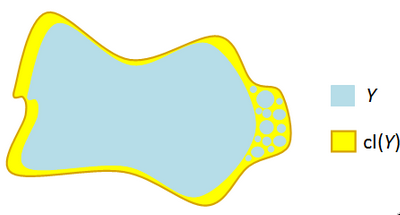
\includegraphics[width=0.8\textwidth]{assets/closure_ex.png}
  \caption{Closure of a Set}
  \label{fig:closure_ex}
\end{figure}

\begin{prop} $\overline{E} = E \cup E'$ (where $E'$ is the set of limit points of  $E$) 
  \begin{proof} We will first prove $E \cup E'$ closed. Take $x \in X \cup E'$.Then,  $x$ is not 
         an limit point of  $E \to \exists r >$ such that $B_r^{0} (x) \cap E = \emptyset$. 
         Since $x \not\in E \to B_r(x) \cap E = \emptyset$ $\to E \subseteq X \setminus B_r(x)$ and $X \setminus B_r(x)$ is closed
         since it is the complement of $B_r(x)$ which is open (all balls are open) in $X$. Then 
         $E' \subseteq [X \setminus B_r(x)]' = X \setminus B_r(x)$ and $E' \cap B_r(x) = \emptyset$.
         Hence, $B_r(x) \cap (E \cup E') = \emptyset$ or equivalently,
          \[
         B_r(x) \subseteq X \setminus (E \cup E')
         .\]
         We know that $X \setminus (E \cup E')$ must be open since an open set $B_r(x)$ is contained in it,
         so,
          \[
         E \cup E'
         \]
         is a closed set.\\ 

         Then, we will show  $E \cup E' \supseteq \overline{E}$
         \[
         E \cup E' \supseteq E \to E \cup E' \supseteq \overline{E}
         .\] 
         by property (3) in the definition since $E \cup E'$ is closed. \\


         For the other direction, 
         \[
           \overline{E} \supseteq E \to \overline{E}' \supseteq E' 
         .\] 
         since $\overline{E}' \subseteq \overline{E}$,
         \[
         \overline{E}' \supseteq E' \to \overline{E} \supseteq E'
         .\] 
         and by property (6). So, 
         since $\overline{E} \supseteq E$ and $\overline{E} \supseteq E'$ :
         \[
         \overline{E} \supseteq E \cup E'
         .\] and with both directions proven, 
         \[
         \overline{E} = E \cup E'
         .\] 
  \end{proof}
\end{prop}

\section{Sequences}
\begin{definition}
  Take $\left( X, \rho \right) $ a metric space. A \textbf{sequence} $\{x_n\}_{n \geq 1} $ is a map
  \begin{align*}
     \N &\longrightarrow X  \\
     n &\longmapsto x_n  
  .\end{align*}
  The \textbf{image (range)} of a sequence, 
  \[
    im(\{x_n\}_{n \geq 1}) = \{x \in X | \exists k \geq 1 \text{such that} x_k = x\} 
  .\]
\end{definition}

\begin{note}{Example}\\
  Consider 
  \[
  x_n = \begin{cases}
    1, \text{ n even} \\
    0, \text{ n odd}
  \end{cases}
  .\] so $x_1=0, x_2 = 1, x_3=0, \ldots$. Then the range would be
  \[
  im\left( \{x_n\}_{n \geq 1}  \right) = \{0,1\} 
  .\] 
\end{note}


\begin{definition}
  Let $\{x_n\}_{n \geq 1}$ a sequence in $X$. We say that $x \in X$ is the \textbf{limit} of this sequence if
  $\forall \epsilon > 0$,  $\exists N \geq 1$ such that $\forall n \geq N$ we have that 
   \[
  x_n \in B_\epsilon (x)
  .\] 
  In this case we can say that $\{x_n\}_{n \geq 1}$ converges to $x$ as  $n \to \infty$. We write:
  \[
  x_n \to x (n \to \infty)
  .\]
  or equivalently
  \[
  \lim_{n \to \infty} x_n = x
  .\] 
  Note that we sometimes have to specify the metric space if $x_n$ is in multiple metric spaces. The image must always be \textbf{countable} (even if the sequence converges to $x \in \R$ because the indices we map from are countable $\N$) 
\end{definition}

\begin{note}{Example} \\
  The previous example does not have a limit because $x_n$ oscillates so the "tail" is never contained
  around  $0$ or $1$ for any  $\epsilon$, because the next  $x_{i+1}$ flips the parity so it "jumps"
  and is not contained in that $B_{\epsilon}(x)$ ball.
\end{note}

\begin{prop}
  If $x', x''$ are limits of  $\{x_n\}_{n \geq_1}$ then $x' = x''$ (i.e. the limit is unique)
\end{prop}

\begin{prop}
  If $\{x_n\}_{n \geq 1}$ converges, then $im(\{x_n\}_{n \geq 1}$ is a bounded set in $X$
\end{prop}

\subsection{Subsequence}
\begin{definition}
  Let $\{x_n\}_{n \geq 1}$ be a sequence and $1 \leq n_1 < n_2 < \ldots < n_k < \ldots$, i.e $n_j \in \Z$ where $j \geq 1$, then we get  $\{x_{n_j}\}_{j \geq 1} $ is a \textbf{subsequence} of $\{x_n\}_{n \geq 1} $.
\end{definition}

\begin{prop}
  If $x_n \to x$ as  $n \to \infty$, then any subsequence  $\{x_{n_j}\}_{j \geq 1} $ converges to $x$. 
\end{prop}

\begin{theorem}
  Let $(X, \rho)$ be a compact metric space and let  $\{x_n\}_{n \geq 1} $ be a sequence in $X$. Then  $\exists $ 
  a subsequence $\{x_{n_j}\}_{j \geq 1} $ and $x \in X$ such that this  $x_{n_j} \to x$ as $j \to \infty$ (In other words, every sequence in a compact metric space has a convergent subsequence.)

  \begin{proof}
    Let us first assume that $im(\{x_n\}_{n \geq 1}) $ has finitely many elements: $y_1, y_2, \ldots, y_n (y_k \neq y_j$ if $k \neq j$). Then, $\exists \{x_{n_j}\}_{j \geq 1} $ and $1 \leq l \leq N$  such that $x_{n_j} = y_l$ $(\forall j \geq 1)$ (this is true by pigeonhole principle, finite $y_l$, infinite  $x_{n_j}$, so at least one distinct value for $y_l$ must appear infinitely in the sequence $\{x_n\}$, then this guarantees there is some subsequence $\{x_{n_j}\}_{j \geq 1} $ whose terms are equal to a fixed $y_l$). Then, clearly $x_{n_j} \to y_l$ as $(j \to \infty)$. \\


    Now assume that the range of $\{x_n\}_{n \geq 1} $ is not finite. Let $S = im(\{x_n\}_{n \geq 1}) $. Since $X$ is compact and $S \subseteq X$ has infinitely many points. We can use the proposition from the previous lecture, which tells us that  $\exists x \in X$ that is a limit point of this set. Define a ball centered at $x$. 
    \[
    B_{\frac{1}{n}} (x) n \geq 1
    .\] 
    For $n = 1$,  $\exists x_{n_1}, n_1 \geq 1$ such that $x_{n_1} \in B_1 (x)$. For $n=2$, $\exists x_{n_2}$, $n_2 > n_1$ such that  $x_{n_2} \iin B_{\frac{1}{2}} (x)$. \ldots For $n = k \exists  x_{n_k}, n_k > n_{k-1}$ such that $x_{n_k} \in B_{\frac{1}{k}}(x)$ (by definition of limit point). Then, $x_{n_j} \to x$ as $j \to \infty$ 
  \end{proof}
\end{theorem}

\subsection{Diameter}

\begin{definition}
 Let $(X, \rho)$ a metric space.  $E \neq \emptyset \subseteq X$ and  $E$ bounded. The we can defined
 \[
diam(E) = \sup \{\rho(x,y) \mid x,y \in E \} 
.\] 
Can be thought of as the max distance between two points in the set $E$ i.e. the diameter. 
\end{definition}
\begin{lemma}
Let $E \subseteq X$ be a bounded set. Then, 
\[
diam \overline{E} = diam E
.\] 

\begin{proof}
  Since $\overline{E} \supseteq E \to diam \overline{E} \geq diam E$. \\


  Take $x,y \in \overline{E} = E \cup E' \to \forall \epsilon > 0$, $\exists x',y' \in E$ such that $\rho(x,x') < \epsilon$ and $\rho(y,y') < \epsilon$. Here we say that x and y are either an element of $E$ or a limit point of  $E$ so they are  $\epsilon$ close to $x,y$ respectively. Then by the triangle inequality (applied twice), 
 \begin{align*}
   \rho(x,y) &\leq  \rho(x,x') + \rho(x',y') + \rho(y',y) \\
             &< \epsilon + diam(E) + \epsilon \\
             &< diam(E) + 2\epsilon
 .\end{align*}
 Hence for any $x,y \in \overline{E}$, $\forall \epsilon > 0$ we have that:
  \[
 \rho(x,y) < diam(E) + 2 \epsilon
 .\]
 For fixed $\epsilon$ and any x,y
 \[
 diam(\overline{E}) \leq diam(E) + 2 \epsilon
 .\] 
 From here follows (a bit counterintuitive but consider if $a \leq b + \epsilon$ was not true),
 \[
 diam \overline{E} \leq diam(E)
 .\] \\

 As $diam \overline{E} \geq diam E$ and $diam \overline{E} \leq diam E$, then $diam \overline{E} = diam E$
\end{proof}
\end{lemma}
\begin{note}
  For $diam(\overline{E})$ to even be a valid question, $\overline{E}$ must be bounded so we use the fact that the closure of a bounded set is always bounded.
\end{note}

\subsection{Cauchy Sequence}
\begin{lemma}
  Let $K_1 \supseteq K_2 \supseteq \ldots \supseteq K_j \supseteq \ldots$ where $K_j \neq \emptyset$ are compact sets in $X$. Then,  $\cap_{j \geq 1} K_j \neq \emptyset$
  \begin{proof}
    Consider 
    \[
    G_j = X \setminus K_j, j \geq 1
    .\]
    Since $K_j$ is compact, then it is closed, so  $G_j$ is open $\forall j \geq 1$.  Assume that all conditions in the lemma hold but $\cap_{j \geq 1} K_j = \emptyset$. Then, 
    \[
      \cup_{j \geq 1} G_j = \cup_{j \geq 1} \left( X \setminus K_j \right) =X \setminus [\cap_{j \geq 1} \left( X \setminus (X \setminus K) \right)]= X \setminus [\cap_{j \geq 1} K_j] =   
    .\] 
    TODO

  \end{proof}
\end{lemma} 
Let $\left( X, \rho \right) $ a metric space, $\{x_n\}_{n \geq 1} $ is a sequence in $X$

\begin{definition}
  $\{x_n\}_{n \geq 1} $ is a \textbf{Cauchy sequence} if and only if  $\forall \epsilon > 0$ $\exists N \geq 1$ such that 
  \[
    \forall n,m \geq N, \rho(x_n,x_m) < \epsilon
  .\] 
  An example would be an asymptote that doesn't go to infinity. A cauchy sequence must be a \textbf{bounded set}, or more precisely the range of the cauchy sequence must be \textbf{bounded} 
\end{definition}

\begin{note}
  Notice that the difference in defintion between cauchy and limit is that cauchy doesn't assume the existence of $x$ such that  $x_n \to x$. Usually, a cauchy is used to find $x$ and show it exists. So cauchy sequence  $\supseteq$ convergent sequence 
\end{note}

\begin{note}{CounterExample}\\
  A cauchy sequence in a metric space that does not converge (i.e. the metric space is not complete).\\


  Consider $X = [0,1) \subseteq \R$ with standard $\rho$. Take  $x_n = 1 - \frac{1}{n}, n \geq 1$. Then this sequence is a cauchy sequence in $\R$ and since distance is inherited by $X$, then  the sequence is also cauchy in  $X$. However, while the $\{x_n\}_{n \geq 1} $ converges in  $\R$, it does not converge in $X$.   
\end{note}

\begin{definition}
  A metric space $\left( X,\rho \right)  $ is \textbf{complete} $\iff$ any cauchy sequence in  $X$ converges to some point  $x \in X$.  
\end{definition}

\begin{prop}
  If $x_n \to x$ as  $n \to \infty$  then $\{x_n\}_{n \geq 1} $ is a cauchy sequence.

  \begin{proof}
    
  \end{proof}
\end{prop}

\begin{prop}
 If $\{x_{n}\}_{n \geq 1}$ be a cauchy sequence then $im(\{x_n\}_{n \geq 1})$ is bounded (the same as saying the sequence is bounded) 
 \begin{proof}
   
 \end{proof}
\end{prop}

\begin{prop}
  $\{x_n\}_{n \geq 1} $ is a cauchy sequence $\iff$ $diam\left( \{x_n\}_{n \geq N}  \right) \to 0$ as $N \to \infty$ (by the previous proposition we know that $\{x_n\}_{n \geq N} $ is bounded, so the diam is well-defined)  

  \begin{proof}
    $\to$ Assume that  $\{x_n\}_{n \geq 1} $ is a cauchy sequence then $\forall \epsilon$  $\exists N \geq 1$ such that $\forall m,n \geq N, \rho(x_n,x_m) < \epsilon$. Notice that this means $diam(\{x_n\}_{n \geq N}) \leq \epsilon$ (the tail of the sequence is contained in a ball of radius $\epsilon$). Hence,  $\forall \epsilon > 0$,  $\exists  N \geq 1$ such that $k \geq N$,
    \[
    diam\left( \{x_n\}_{n \geq k}  \right) \leq \epsilon \iff diam\left( \{x_n\}_{n \geq k}  \right) \to 0 (k \to \infty) 
    .\] 

    $\leftarrow$ Assume that $diam\left( \{x_n\}_{n \geq N}  \right) \to 0$ as $N \to \infty$ then $\forall \epsilon > 0$, $\exists N_0 \geq 1$ such that $\forall N \geq N_0$, we have  $diam(\{x_n\}_{n \geq N}) < \epsilon $. (We are now looking at $B_\epsilon^{\R}(0) = (-\epsilon, \epsilon)$ and saying the diameter is a element in this ball). This implies that $\forall m,n \geq N$, 
    \[
    \rho(x_n, x_m) < \epsilon
    .\] 
    Then $\forall \epsilon > 0$,  $\exists N_0 \geq 1$ such that $\forall m,n \geq N_0$. Hence, $\{x_n\}_{n \geq 1} $ is a cauchy sequence.   
  \end{proof}
\end{prop}

\begin{theorem}
  If $X$ is compact  $\to$  $X$ is complete. (but not the other way around)

  \begin{proof}
    Assume that $X$ is compact. Take a cauchy sequence  $\{x_n\}_{n \geq 1} $ in $X$. Consider the tail of this sequence, 
    \[
    E_N = \{x_n\}_{n \geq N}, N = 1,2,3,\ldots 
    .\] 
Then, 
\begin{enumerate}
  \item $E_1 \supseteq E_2 \supseteq \ldots \supseteq E_N \supseteq \ldots$
  \item For any $N \geq 1$,  $E_N$ is a bounded set and  $diam(E_N) \to 0$ as  $N \to \infty$ since  $E_N$ is a subsequence (relative order maintained) of  $\{x_n\}_{n \geq 1} $ then it is also cauchy and we can apply the proposition.
\end{enumerate}
Hence, by taking the closure,
\[
X \supseteq \overline{E_1} \supseteq \overline{E_2} \supseteq \ldots \supseteq \overline{E_N} \supseteq \ldots 
.\] 
and each $\overline{E_i}$ is closed and we proved that closed subsets of compact sets are also compact, so  $\overline{E_i}$ are also compact in  $X$. On the other side, we have
\[
  diam(\overline{E_N}) \leftarrow 0 \text{ as } N \leftarrow \infty
.\] 
by lemma 1 (since we know $diam(\overline{E}) = diam(E)$). It follows from before that $\cap_{j \geq 1} K_j \neq \emptyset \to  \exists x \in X,$ such that $x \in \overline{E_N}$, $\forall N \geq 1$ (it is in the intersection). This means $\forall \epsilon > 0$,  $\exists N_0 \geq 1$ such that $\forall N \geq N_0$, 
\[
diam(\overline{E_N}) < \epsilon \to diam(\overline{E_{N_0}}) < \epsilon \to \rho(x, x_n) < \epsilon,  \forall n \geq N_0
.\] 
Hence, $\forall \epsilon > 0, \exists  N_0 \geq 1$ such taht $\forall n > N_0$,
 \[
\rho(x,x_n) < \epsilon \iff x_n \in B_{\epsilon} (x), \forall n \geq N_0
.\] 
Thus,
\[
  x_n \to x \text{ as } n \to \infty 
.\] 
  \end{proof}
\end{theorem}

\begin{theorem}
  $\R^{n}$ is complete (observe that $\R^{n}$ is not compact so we can't use the theorem above). Note that this proof does not hold for infinite dimensional spaces.

  \begin{proof}
    Take a cauchy sequence in $\R^{n}$, $\{x_n\}_{n \geq 1} $. Let $S = range(\{x_n\}_{n \geq 1})$. Thus, $S \neq \emptset$ and  $S$ is bounded. Consider $\overline{S}$. Then, $\overline{S}$ is closed and bounded subset of $\R^{n}$ so $\overline{S}$ is compact in $\R^{n}$ (Note we only proved this for $\R^{n}$ ). Then, $\{x_{n}\}_{n \geq 1} $ is a cauchy sequence in $(\overline{S}, \rho)$ (as $\overline{S}$ contains all of $\{x_n\}_{n \geq 1} $). Now we have a compact metric space and a cauchy sequence, so by theorem 1, $\exists  x \in \overline{S}$ such that in $\overline{S}$ 
    \[
      x_n \to x \text{ as } n \to \infty 
    .\] 
    this implies
    \[
      x_n \to x \text{ as } n \to \infty
    .\] 
    in $X$!
  \end{proof}
\end{theorem}

\end{document}



